\documentclass[10pt]{beamer}

\usepackage{amsfonts}
\usepackage{subfiles}
\usepackage[T2A]{fontenc}
\usepackage[utf8]{inputenc}
\usepackage[russian]{babel}

\usepackage{amsmath, amsfonts, amssymb, amsthm, mathtools, mathrsfs}
\usepackage{wasysym, dsfont}
\usepackage{graphicx}
\usepackage{float}
\usepackage{wrapfig}
\usepackage{subcaption}
\usepackage{multirow}
\usepackage{caption}
\usepackage{subcaption}
\usepackage{longtable}
\usepackage{subfigure}

\usepackage{multicol}
\DeclareMathOperator*{\argmax}{\arg\!\max}
\DeclareMathOperator*{\argmin}{\arg\!\min}

\mode<presentation>
{
	\usetheme{boxes}
	\beamertemplatenavigationsymbolsempty
	
	\setbeamertemplate{footline}[page number]
	\setbeamersize{text margin left=1.5em, text margin right=2.0em}
}
\newcommand\blfootnote[1]{%
	\begingroup
	\renewcommand\thefootnote{}\footnote{#1}%
	\addtocounter{footnote}{-1}%
	\endgroup
}
\newcommand\FontUP{\fontsize{12}{12}\selectfont}


\title[]{Rethinking Parameter Counting in Deep Models:
Effective Dimensionality Revisited}

\author{Nikita Okhotnikov}
\institute{MIPT}
\date{2024}

\begin{document}

\begin{frame}
  \titlepage
\end{frame}


\begin{frame}
    \frametitle{Introduction}
    \begin{itemize}
        \item Number of parameters -- poor generalisation metric
        \item Effective dimensionality might be a better one
        \item There's a connection to variance of posterior distribution
    \end{itemize}
\end{frame}

\begin{frame}
    \frametitle{Theory behind}
    \begin{block}{Posterior Contraction:}
    $$\Delta_{post}(\theta) = tr(Cov_{p(\theta)}(\theta)) - tr(Cov_{p(\theta|\mathcal{D})}(\theta))$$
    \end{block}
    \begin{block}{For Bayesian linear regression:}
    \vspace{-0.2cm}
    $$\Delta_{post}(\theta) = \alpha^2\sum_{i=1}^N \frac{\lambda_i}{\lambda_i + \alpha^{-2}}$$
    \end{block}
    \vspace{-0.2cm}
    \begin{block}{Params vs functions distribution}
        \begin{center}
            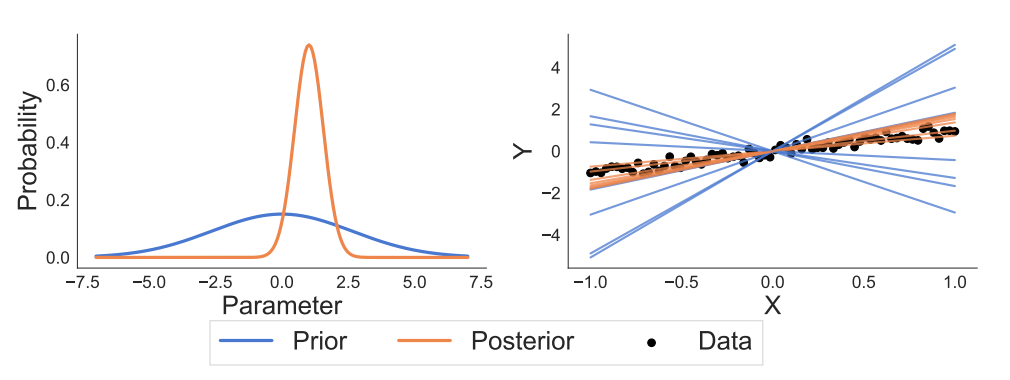
\includegraphics[scale=0.4]{Params_and_functions_distributions.png}
        \end{center}
    \end{block}
\end{frame}


\begin{frame}
    \frametitle{Theory behind}
    \begin{block}{Effective Dimensionality of symmentric matrix $A\in \mathbb{R}^{k\times k}$:}
    $$N_{eff} (A, z) = \sum_{i=1}^k \frac{\lambda_i}{\lambda_i + z} \text{, where } \lambda_i \text{ -- eigenvalues of A and } z > 0$$
    \end{block}
    \begin{block}{Laplace approximation}
    \vspace{-0.5cm}
    $$\theta_{MAP} = \argmax_\theta p(\theta|\mathcal{D}),~~\theta\sim\mathcal{N}(\theta_{MAP}, (\mathcal{H}_\theta + A)^{-1}),$$
    $$\text{where } A = -\nabla\nabla_\theta\log p(\theta),~~~ \mathcal{H}_\theta = -\nabla\nabla_\theta \mathcal{L}(\theta, \mathcal{D}) =\nabla\nabla_\theta\log p(\theta|\mathcal{D})$$
    \begin{center}
        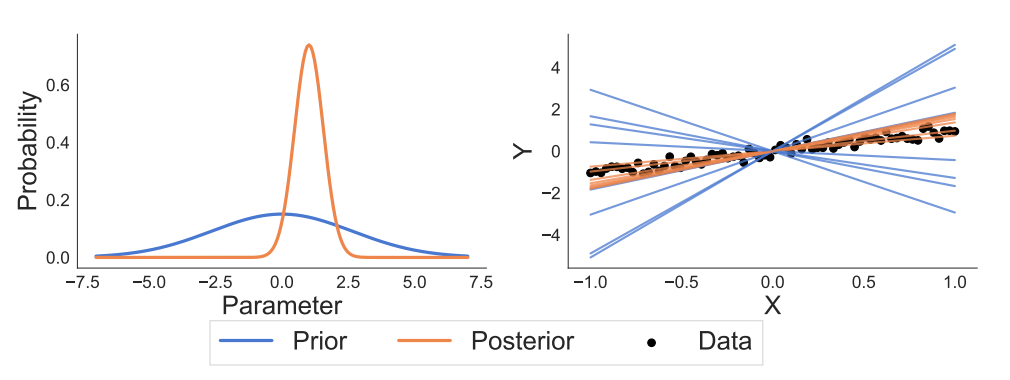
\includegraphics[scale=0.4]{Params_and_functions_distributions.png}
    \end{center}
    \end{block}
    
\end{frame}

\begin{frame}
    \frametitle{Posterior contraction and effective dimensionality}
    \begin{block}{Theorem}
        $\Phi = \Phi(x)\in \mathbb{R}^{n\times k}$ -- feature map of $n$ observations, $n<k$. \\
        $\beta \sim \mathcal{N}(0_k, \alpha^2, I_k)$ -- parameters prior. \\
        Model -- $y\sim \mathcal{N}(\Phi\beta, \sigma^2I_n)$.\\
        Then the posterior distribution of $\beta$ has a $k-n$ directional subspace in which the variance is identical to the prior variance.
    \end{block}
    
\end{frame}

\begin{frame}
    \frametitle{Posterior contraction and effective dimensionality}
    $$\Phi = \Phi(x)\in \mathbb{R}^{n\times k} = \left[\cos(\pi x), \sin(\pi x), \cos(2\pi x), \sin(2\pi x)\dots \right], ~~\beta\sim \mathcal{N}(0, I)$$
    $$\text{ground truth parameters }\beta^* \text{from the same distribution. } y\sim \mathcal{N}(\Phi\beta, \sigma^2 I)$$
    \begin{center}
        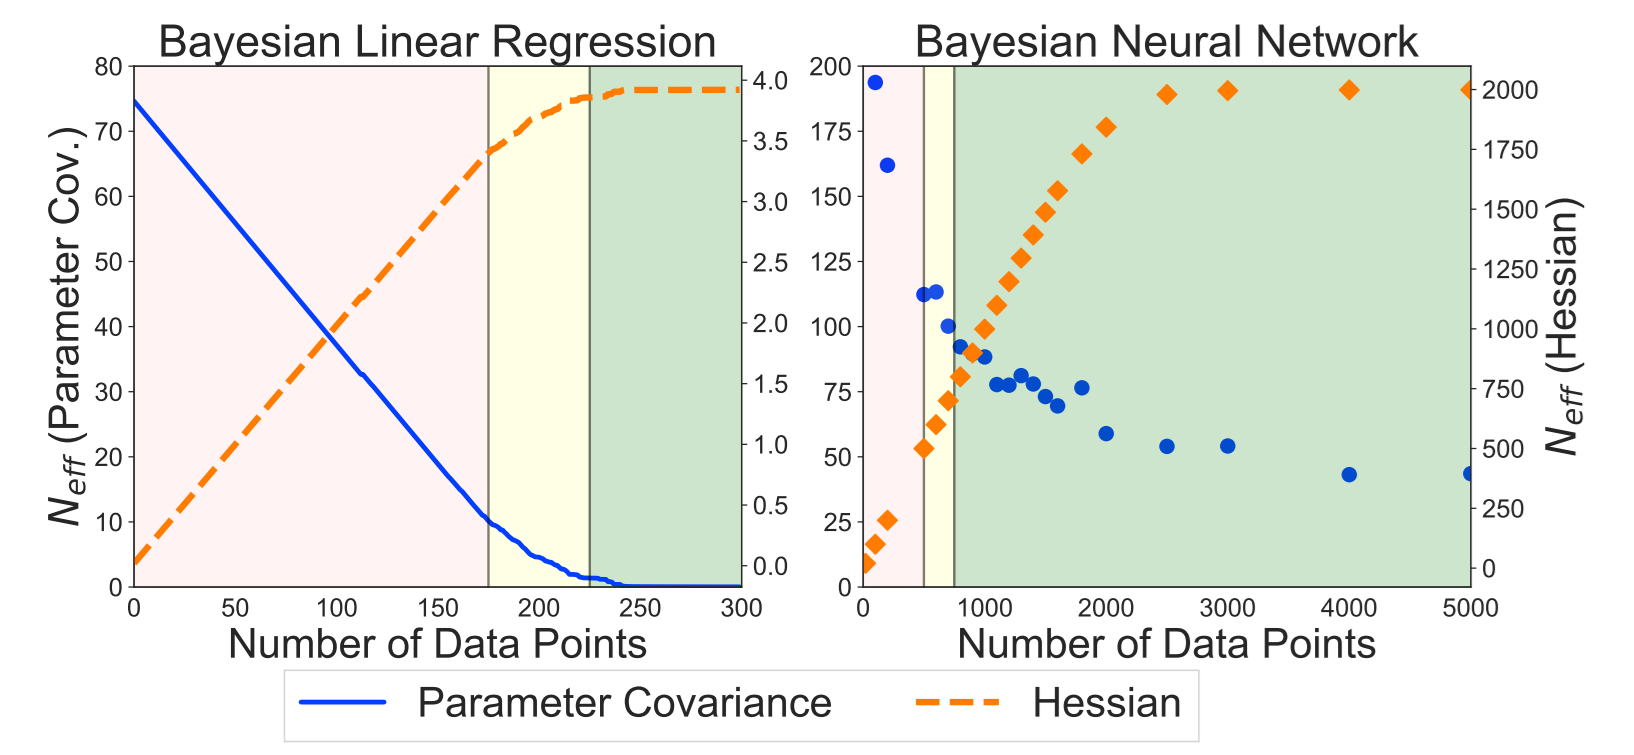
\includegraphics[scale=0.27]{ridge_dimensionality_and_variance.png}
    \end{center}
    
\end{frame}

\begin{frame}
    \frametitle{Function-space homogenenity in linear models}
    \begin{block}{Theorem}
        $\Phi = \Phi(x)\in \mathbb{R}^{n\times k}$ -- feature map of $n$ observations, $n<k$.\\
        $\beta \sim \mathcal{N}(0_k, \alpha^2, I_k)$ -- parameters prior.\\
        The minimal eigenvectors of the Hessian define a $k - n$ dimensional subspace in which parameters can be perturbed without changing the training predictions in function space. (Proved for generalized linear models)
    \end{block}
    \begin{center}
        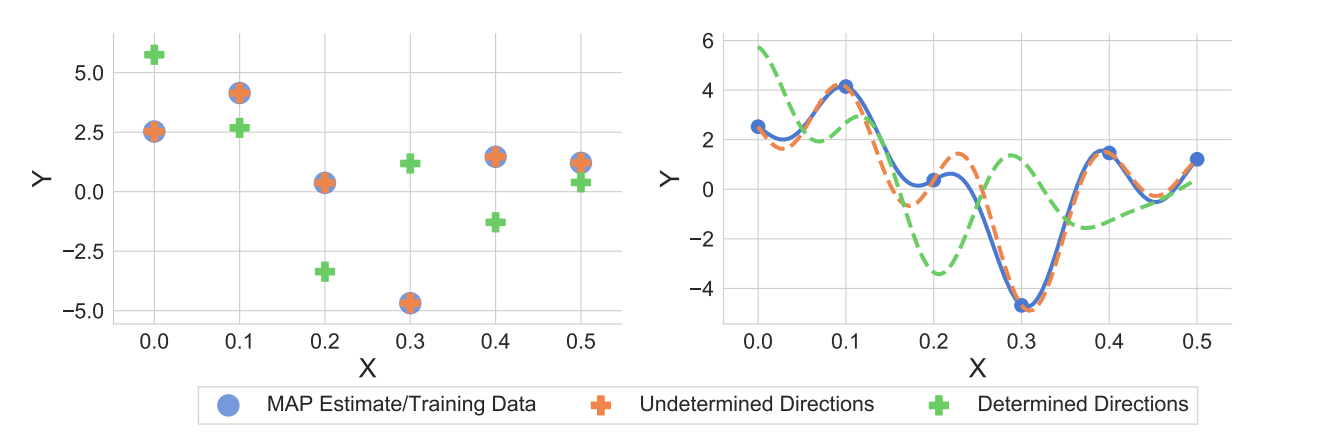
\includegraphics[scale=0.35]{disturb_params.png}
    \end{center}
\end{frame} 

\begin{frame}
    \frametitle{Loss Surfaces in Orthogonalized basis}
    \begin{center}
        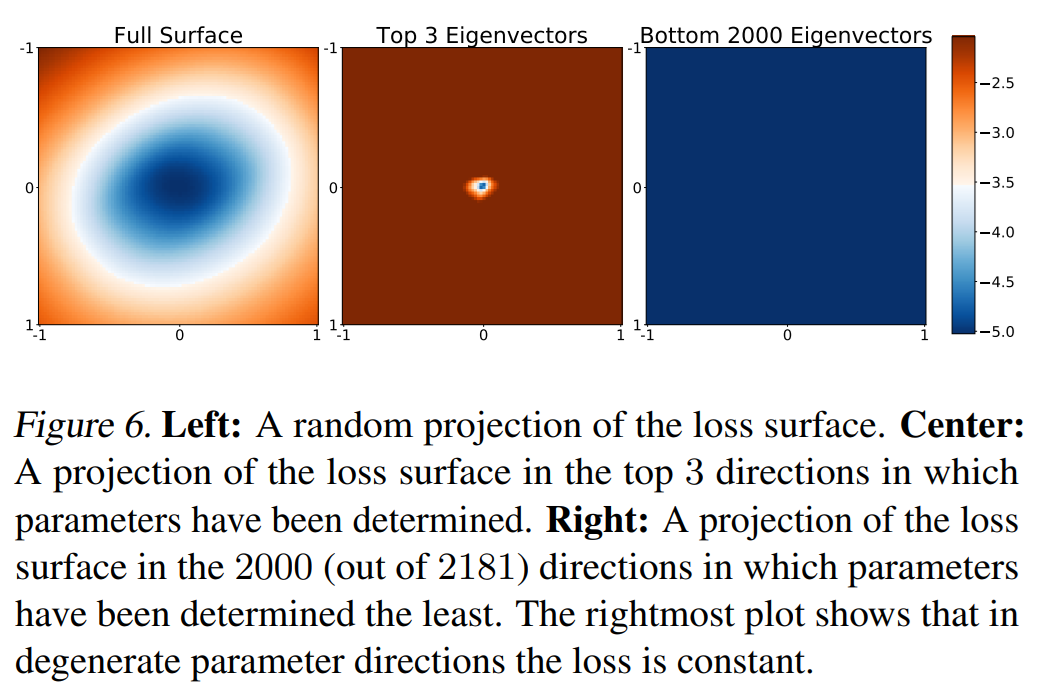
\includegraphics[scale=0.35]{LossProjection.png}
    \end{center}
\end{frame}

\begin{frame}
    \frametitle{Degenerate Parameters Lead to Homogeneous Models}
    Perturbing some parameters in over-parameterized model leads to model equivalent in function space
    $$\theta \longleftarrow \theta^* + s\frac{Bv}{\|Bv\|_2}, ~~v\sim \mathcal{N}(0, I_d), ~B \text{ -- d-dimensional basis}, ~~s \leqslant\|\theta^*\|_2/2$$
    \begin{center}
        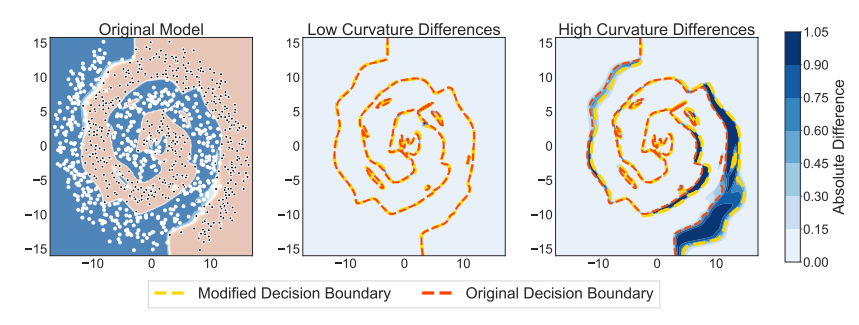
\includegraphics[scale=0.4]{perturb_params_classification.png}
    \end{center}
    Thus, we might probably ignore subspaces of degenerate parameters for model compression.
\end{frame}

\begin{frame}{Effective dimensionality and compression}
    \begin{center}
        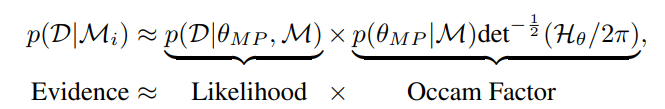
\includegraphics[scale=0.4]{eq6.png}
    \end{center}
    Lower eigenvalues $\rightarrow$ lower effective dimensionality and higher Occam Factor $\rightarrow$ lower description length and better compression 
    \begin{center}
        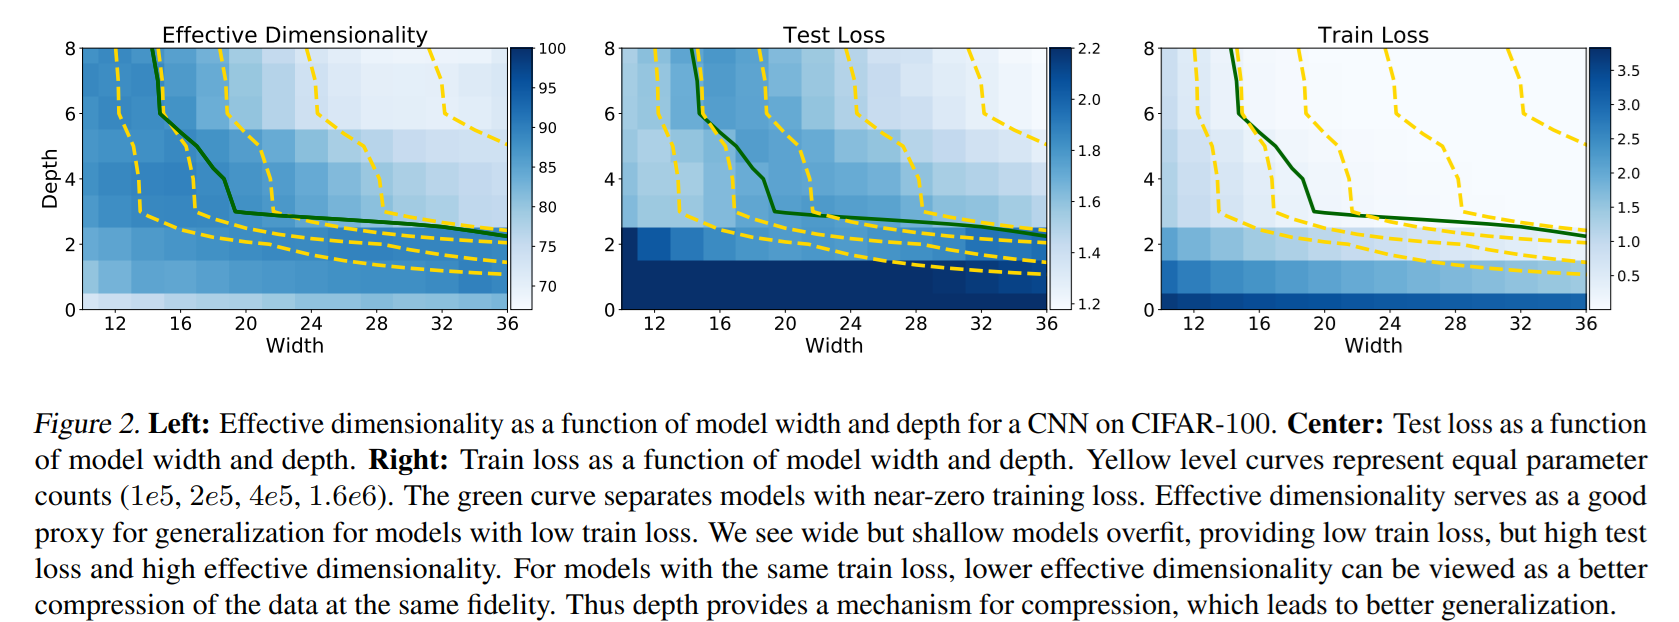
\includegraphics[scale=0.26]{model_sizes.png}
    \end{center}
\end{frame}

\begin{frame}{Effective dimensionality and generalization}

    \begin{center}
        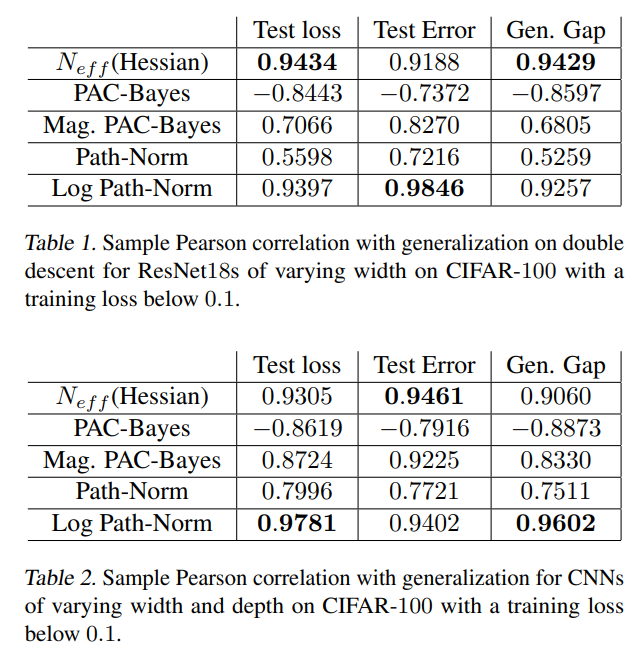
\includegraphics[scale=0.43]{generalisation_metrics.png}
    \end{center}
\end{frame}



\end{document}